\documentclass[conference, 11pt]{IEEEtran}
\IEEEoverridecommandlockouts
% The preceding line is only needed to identify funding in the first footnote. If that is unneeded, please comment it out.
\usepackage[noadjust]{cite}
\usepackage{amsmath,amssymb,amsfonts}
\usepackage{algorithmic}
\usepackage{graphicx}
\usepackage{textcomp}
\usepackage{xcolor}
\usepackage{subcaption}
\usepackage{booktabs, caption, tabularx, makecell}
\usepackage{multirow}
%\usepackage{biblatex}
\def\BibTeX{{\rm B\kern-.05em{\sc i\kern-.025em b}\kern-.08em
T\kern-.1667em\lower.7ex\hbox{E}\kern-.125emX}}
\setcellgapes{4pt}

\begin{document}

    \title{Machine Learning Approaches for Detection of DoS Attacks in IoT Networks\\}

    \author{\IEEEauthorblockN{Adrian Gruszczynski}
    \IEEEauthorblockA{\textit{Freie Universit\"at Berlin} \\
    IoT \& Security Seminar Report}}

    \maketitle

    \begin{abstract}
        Internet of Things (IoT) is a rapidly growing market estimated to house over 50 billion connected devices by 2020.
        At its core, IoT allows connecting everyday objects to create smart devices capable of sensing the surrounding environment and processing data to make decisions without human intervention.
        It has a broad range of potential applications in domains such as smart home, healthcare, logistics, manufacturing, etc.
        Due to limited computational resources and energy consumption, only rudimentary firmware runs on the devices.
        In recent years, a range of distributed denial of service attacks (DDoS) powered by IoT botnets demonstrated the scale at which critical internet infrastructure is affected.
        Consequently, researchers around the world started investigating this phenomenon.
        This study presents an overview of machine learning methods for DDoS detection in the context of practical application.
        It provides the necessary background for understanding the IoT ecosystem, DDoS and machine learning methods, followed by a detailed explanation of two concrete approaches.
        The study finishes with a comparative analysis of DDoS detection techniques for IoT.
        Although machine learning for DDoS detection shows high potential, there is room for improvement in the context of practical implementation.
    \end{abstract}

    \begin{IEEEkeywords}
        DDoS, IoT, anomaly detection, machine learning, botnet
    \end{IEEEkeywords}


    \section{Introduction}
    Internet of Things is a group of heterogeneous physical devices running software, often equipped with sensors that exchange data with other devices over the Internet or other communication networks \cite{article:4}.
    The networking and computing capabilities are limited due to size, space and energy consumption constraints.
    It facilitates automation by measuring and recognising events from the near surroundings.
    There are countless use-cases for IoT in various domains, including consumer electronics, smart cities and healthcare \cite{article:1}.
    Nowadays, IoT is an interdisciplinary area of research involving numerous fields such as Machine Learning, Embedded Systems, Networking and Distributed Systems.
    It facilitates automation, control of the environment and intelligent decision-making that requires low human intervention and thus enjoys wide popularity and adoption.
    Due to the variety of use-cases and application domains, the IoT ecosystem consists of a substantial number of diverse standards and technologies adapted within the network.
    Critics emphasise security and privacy concerns as the primary weak spot of IoT.
    In the upcoming years, the number of connected IoT devices will increase significantly, resulting in higher decentralisation and complexity, causing further fragmentation within the ecosystem.
    The emergence of a new application layer called Web of Things and the application of modern machine learning techniques will open a market for novel services that might adapt to individual human needs.

    Thanks to the wide adoption, IoT devices are very close to humans and can affect our well-being and safety.
    Furthermore, a variety of critical systems and infrastructure depends on these devices.
    The great interest and predicted future adoption make IoT an active area of research that attracts scientists from outside of computer science and electrical engineering, for instance, social sciences or environmental studies.
    The enormous number of connected devices poses a significant security threat and provides a vector for potential misuse.
    In particular, the propagation of insecure IoT devices offers a fertile ground for malicious actors and has resulted in multiple distributed denial of service (DDoS) attacks on critical internet infrastructure \cite{article:16}, \cite{article:8}.
    To address this issue, scientists propose various solutions, including Machine Learning techniques.
    Machine learning (ML) provides methods for detecting patterns in data and enjoys ever-increasing popularity.
    Modern applications leverage Machine Learning for translation, speech recognition and computer vision \cite{Goodfellow-et-al-2016}.
    In the cyber-security field, Machine Learning finds use for fraud, malware and spam detection \cite{article:18}.
    With the recent emergence of deep learning, strategical reasoning and decision-making of a machine may exceed human performance creating room for novel use-cases.
    The application of modern Machine and Deep Learning approaches delivers a toolbox for network traffic analysis, intrusion detection and real-time anomaly detection.
    Thanks to the variety of use-cases and the fragmentation within the IoT ecosystem, a broad implementation of Machine Learning methods for DDoS detection stays challenging.
    Further limitations such as limited computing resources, energy constraints and complex system architecture call for novel solutions.

    The aim of this study is to evaluate several Machine Learning approaches for DDoS detection in the context of practical implementation within the IoT ecosystem.
    It will highlight various strategies for DDoS detection in IoT systems to explore the current state of the art and explain one method in more detail.
    The objective is to improve the understanding of DDoS detection in IoT and demonstrate the role of machine learning.


    \section{Related Work}
    The application of machine learning approaches for DDoS detection in IoT is an emerging area of research.
    Although DDoS detection in IoT and DDoS detection with machine learning are both well-researched fields, the body of research on applying machine learning approaches for DDoS detection in IoT leaves much to be desired.
    To my knowledge, there is no survey comparing machine learning and Deep Learning methods for DDoS detection under IoT constraints.
    Specifically, the practical aspects of these methods, such as computational complexity, energy consumption, ability to detect unknown attacks and detection performance, are unexplored and will benefit from further examination.
    The existing surveys focus on general DDoS attacks and defences in IoT or provide a broader perspective on various machine learning methods for IoT Security.

    \subsection{General DDoS Protection}
    In the general DDoS protection and prevention field, R. Vishwakarma and A. K. Jain present a comprehensive survey of DDoS attacks and DDoS defence techniques for IoT \cite{article:14}.
    They introduce the layered IoT architecture and demonstrate the security issues of IoT networks.
    They propose an extensive taxonomy of IoT-specific DDoS attack types and defence techniques.
    Furthermore, they compare the pros and cons of each method and discuss open research questions and limitations.
    Zargar et al., in their survey, propose a taxonomy of DDoS attacks and classify the existing countermeasures for different use-cases \cite{zargar2013survey}.
    They emphasise the role of IoT in the expansion of DDoS attacks.

    \subsection{Machine learning for DDoS protection}
    In the domain of DDoS detection using machine learning methods, Saied et al. apply Artificial Neural Networks (ANNs) to detect and prevent known and unknown DDoS attacks \cite{article:13}.
    They leverage network characteristic data to detect TCP, UDP and ICMP DDoS attacks.
    They obtain training data by reproducing the network environment under DDoS conditions.
    The classification accuracy was superior to existing approaches, particularly for detecting unknown DDoS attacks.
    Ming-Yang Su uses a weighted k-nearest neighbour classifier for real-time DDoS detection \cite{article:2}.
    He proposes a genetic algorithm for feature selection and weighting and evaluates his classifier using several well-known DDoS attacks.
    He obtains 97.42\% detection accuracy for known types of DDoS attacks and 78\% for the unknown.

    \subsection{Machine learning for IoT Security}
    In \cite{cvitic2021novel}, Cvitic et al. propose a conceptual model for DDoS detection in IoT networks based on traffic characteristics.
    They argue that IoT-generated traffic is distinguishable from human-generated network traffic.
    They assign IoT traffic to three categories: periodic updates, event-driven and payload exchange.
    Based on the proposed model, DDoS attacks are an anomaly to the legitimate IoT traffic for a given device type.
    The authors suggest Boosting machine learning method for network traffic anomaly detection.
    Lopez-Martin et al. use flow statistics-based information from the packet header (bytes transmitted, packet interval times, TCP window size, etc.) to develop a network traffic classifier \cite{lopez2017network}.
    They use a dataset of over 250 thousand network flow data points collected from over 100 different services.
    Their classifier combines a Recurrent Neural Network and a Convolutional Neural Network.
    Their best models classify the service (HTTP, Telnet, YouTube, Google, etc.) with 96.23\% accuracy.
    Furthermore, they emphasise the importance of flow data features for classification accuracy.
    Sivanathan et al. show over 99\% accuracy in classifying IoT devices based on patterns in their network activity \cite{sivanathan2018classifying}.
    They collected network traffic data of 28 IoT devices such as cameras, lights and sensors for over six months.
    They present insights into the data using statistical features, propose a state-of-the-art performance multi-stage machine learning classifier and discuss trade-offs of their solution for real-time use.
    Al-Garadi et al. present a survey on Deep Learning methods for IoT Security \cite{article:5}.
    They introduce layers of the IoT system and picture various IoT-specific attack surfaces and threats.
    They review and discuss several machine learning and Deep Learning methods for IoT security in the context of the advantages, shortcomings and opportunities.
    Furthermore, they provide a comprehensive overview of studies applying machine learning and Deep Learning methods on different IoT layers (Perception, Network, Application).
    Finally, they discuss challenges, open issues and future directions for these techniques in IoT security.

    \subsection{Machine learning for DDoS detection in IoT}
    In the field of DDoS detection in IoT networks using machine learning, Aysa et al. investigate the performance of several machine learning approaches for DDoS detection based on network traffic patterns \cite{article:11}.
    The authors use a dataset of actual traffic data collected from 9 commercial IoT devices infected with Mirai and BASHLITE botnets.
    Preliminary results show that combining Decision Trees with a Random Forest outperforms other approaches.
    N. Ravi and S. M. Shalinie examine DDoS attacks triggered by malicious IoT devices on IoT servers \cite{ravi2020learning}.
    They leverage the Software-Defined Network paradigm and semi-supervised machine learning algorithm for DDoS detection and mitigation.
    They reported a 96.28\% accuracy rate in the detection of DDoS attacks.
    In "Boosting-Based DDoS Detection in Internet of Things", Cvitic et al. focus on the IoT-specific DDoS traffic detection model \cite{article:10}.
    They propose an approach for classifying devices into four classes based on the predictability of their network behaviour.
    Their classification accuracy lies between 99.92\% and 99.99\%.
    Doshi et al. demonstrate that IoT-specific network characteristics suffice to detect DDoS attacks with high precision using machine learning methods \cite{inproceedings:1}.
    They conclude that consumer gateway devices could discover local sources of DDoS attacks using low-cost and efficient machine learning algorithms.


    \section{Background and Methods}
    This section consists of two parts: Background and Methods.
    The first part introduces the terminology describing the IoT architecture, types of DDoS attacks, DDoS defence mechanisms and the role of IoT botnets in DDoS attacks.
    The second part comprises an overview of studies on IoT-specific machine learning algorithms for DDoS detection.

    \subsection{IoT Architecture}
    The IoT architecture consists of four primary layers, as shown in Fig. \ref{fig:iota} \cite{article:9}.
    The first layer, called the perception layer, involves physical objects such as sensors, cameras, lightbulbs or microphones.
    The main objective of the physical layer is to collect and store information from the surrounding environment, for instance, motion data, temperature, humidity or acceleration.
    These physical devices operate under the limitations of constrained energy consumption, low computational performance and sparse memory.
    The primary portion of data within the IoT ecosystem comes from this layer.
    The second layer is responsible for connecting heterogeneous IoT devices amongst each other and with the internet.
    The resource limitations of the perception layer force the network layer to optimize for power efficiency, low memory and lossy communication under noisy conditions.
    Covering the variety of use-cases requires different communication protocols, such as 6LoWPAN, WiFi, Bluetooth Low Energy, NFC, ultra-wideband, 3G, 4G etc.
    The third layer, called the middleware layer, provides an abstraction for IoT devices and their connectivity to allow easier application development.
    It facilitates interoperability between heterogeneous IoT devices and takes care of persistence, retrieval and manipulation of data while offering functionality for device discovery, context-aware understanding of sensor data and security.
    Finally, the last layer employs the middleware and provides room for creating a great range of applications in domains such as healthcare, transportation, manufacturing, etc.
    The main objective of the application layer is to present insights from the data to the user and allow user-friendly interaction with the underlying infrastructure.

    \begin{figure}[htbp]
        \centerline{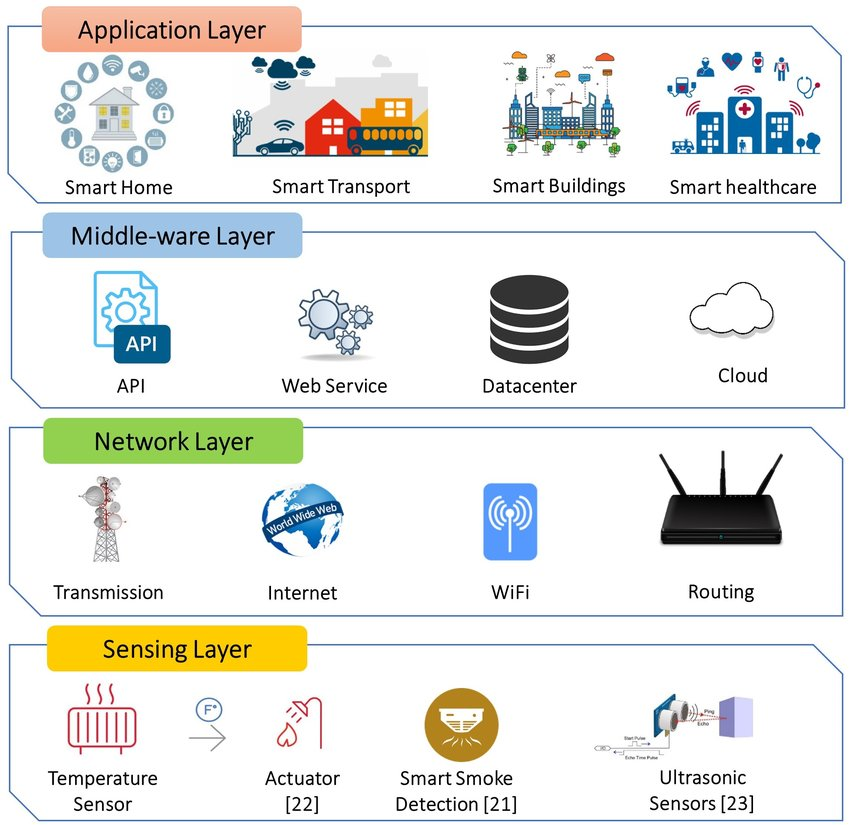
\includegraphics[width=\linewidth]{figures/iot-architecture.jpg}}
        \caption{Architecture of IoT ecosystem consists of four layers \cite{article:9}.}
        \label{fig:iota}
    \end{figure}

    \subsection{Denial of service attacks}
    A denial of service (DoS) attack is a cyberattack in which a cybercriminal seeks to render a host or network resource temporarily unavailable to other users \cite{article:8}.
    DoS attacks work by overwhelming the victim host with a substantial amount of requests, thus, exhausting its resources such as CPU, memory or network bandwidth.
    A distributed denial of service attack (DDoS) is a DoS attack in which the malicious traffic originates from multiple sources.
    These attacks leverage groups of malware-infected, attacker-controlled devices called a botnet.
    DDoS attacks consist of four phases \cite{article:8}:
    \begin{itemize}
        \item Recruitment: in this phase, the attacker performs a scan for a range of IP addresses and searches for vulnerable devices.
        \item Exploitation: the device installs malicious code as instructed by the attacker.
        The installed malware can remove other programs from the device or perform further scans searching for other victims.
        \item Communication: the attacker leverages Command and Control (C\&C) infrastructure to manage the devices and instruct them to perform actions.
        \item Attack: the devices send requests to a specified victim host using fake IP addresses in the packet header to disguise their identity.
    \end{itemize}

    \subsection{Botnets in IoT}
    A botnet is a group of internet-connected devices which execute malware designed to undertake malicious activities such as spamming or DDoS \cite{article:6}.
    The control over a botnet occurs via a dedicated host called botmaster \cite{article:6}.
    Botnet sizes vary from a few hundred to tens or hundreds of thousands of devices.
    Their existence may remain undetected for years.
    IoT devices play a significant role in the effectiveness of DDoS attacks by providing uninterrupted internet connectivity, low-security standards and a large population.
    A recent Linux-based botnet called Mirai \cite{article:16}, \cite{article:6} caused the greatest known DDoS attack, with a flooding rate peaking at 1.2 Tbps.
    The same botnet was responsible for a range of attacks, including an attack on DNS provider Dyn limiting access to services, such as Reddit, Netflix, Twitter and Amazon, across the European Union and the United States \cite{article:8}, \cite{article:16}.
    It operates and propagates in a systematic way, see Fig. \ref{fig:mirai}.
    Mirai scanns IP addresses for IoT devices with exposed Telnet or SSH services and tries brute-forcing the access using a dictionary of default username and password combinations \cite{article:8}, \cite{article:6}.
    In the next step, the C\&C server infects the devices by delivering the malware via FTP or wget for the specific hardware architecture, e.g. ARM, MIPS, Sparc, etc.
    The infected devices become a part of the Mirai botnet and can communicate with the C\&C server.
    The malware loader deletes itself after the installation to avoid detection, and the malware code runs solely in memory.
    The botmaster can instruct the infected devices to perform multiple DDoS attacks or expand the botnet by scanning for additional victims.
    Since the source code for Mirai became open source in 2016, a range of similar variants emerged, all competing for vulnerable devices.

    \begin{figure}[htbp]
        \centerline{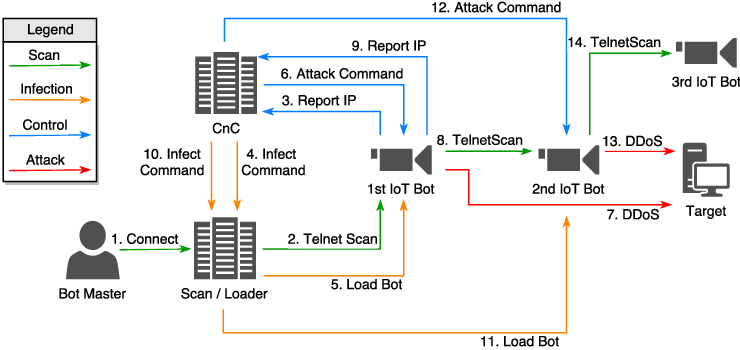
\includegraphics[width=\linewidth]{figures/botnet.png}}
        \caption{Botnet infection and propagation \cite{article:15}.}
        \label{fig:mirai}
    \end{figure}

    \subsection{Classification of DDoS Attacks}
    In practice, simple configuration and hardware constraints of IoT devices, particularly consumer-grade, result in outdated or insecure software and misconfiguration, creating an easy and attractive target for adversaries.
    The amount of always-on vulnerable IoT devices provides an opportunity for launching large-scale DDoS attacks.
    IoT-specific DDoS attacks do not differ much from traditional DDoS attacks and involve diverse and sophisticated techniques \cite{article:14}.
    Due to its nature, preventing DDoS attacks requires identifying limitations and security vulnerabilities in each IoT layer.
    There are two main categories of DDoS attacks: application layer attacks and infrastructure layer attacks \cite{article:14}, \cite{article:8}.
    The application-layer attacks exploit vulnerabilities of web servers or operating systems by leveraging weaknesses in HTTP, DNS or other application-specific protocols.
    The main objective is to exhaust host resources by starting a background process, for instance, sending incomplete POST requests very slowly so that the server runs out of concurrent connections (Slowloris attack) \cite{damon2012hands}.
    The incoming malicious traffic is difficult to tell from the legitimate traffic and thus hard to mitigate.
    IoT botnets play a primary role in application layer attacks by providing a source of legitimate traffic.

    The infrastructure layer attacks exploit vulnerabilities and flaws of the IoT network layer \cite{article:14}, \cite{article:8}.
    They are more popular than application layer attacks.
    This type of attack consists of two categories: volume-based and protocol-based attacks.
    The volume-based attack is the simplest to perform.
    The main goal of a volume-based attack is to overwhelm the victim with the sheer amount of traffic.
    Usually, the attacker employs reflection or amplification techniques for this type of attack.
    The reflection uses forged packets with a fake source IP address for sending requests to a powerful server \cite{article:14}, \cite{article:8}.
    The server responds to these malicious requests and overloads the victim host specified by the fake source IP header with traffic while hiding the attacker's identity.
    The amplification attack uses long server responses combined with IP Spoofing to overwhelm the victim with a large amount of incoming traffic.
    The idea here is that requests are smaller than the server response, e.g. long DNS record, allowing the adversary to magnify the attack scale \cite{article:14}, \cite{article:8}.
    Due to its nature, this attack performs effectively under constrained bandwidth and resources of the IoT devices.
    The protocol-based attack exploits flaws in the network layer to drain the processing capacity of the victim host.
    ACK and SYN flood are well-known protocol-based attacks that exploit the inner workings of the TCP protocol.
    In this attack, the adversary starts the TCP three-way handshake process but does not finish, causing the victim server to wait and consume resources.

    \subsection{DDoS Defence Mechanisms}
    DDoS defence mechanisms comprise two main categories: traditional and IoT-specific DDoS detection \cite{article:14}.
    Traditional DDoS defences run on conventional, homogenous systems and take advantage of powerful resources.
    On the other hand, IoT-specific solutions are more sophisticated and complex due to limited resources and the variety of devices involved.
    Both defence mechanisms rely on monitoring network activity and detection techniques for suspicious traffic.
    Furthermore, there are two subcategories of IoT-specific defence solutions: detection and prevention-based \cite{article:14}.
    The main objective of detection-based defence techniques is to discover the presence of DDoS malware.
    The detection of abnormal activities occurs in the case of traditional DDoS defences on the host or in the network.
    For IoT-based systems, the detection happens primarily in the network.
    DDoS detection works by observing the network traffic and identifying abnormal usage patterns and host behaviour \cite{article:13}.
    If the system discovers any anomalies, it starts to determine the origin of the malicious requests by analyzing individual hosts' behaviour within the network.
    Next, it tries to establish the IP address of the attacker and discards the incoming packets, which alleviates the DDoS attack.
    In the case of IoT networks, the detection system runs on a middlebox or a home gateway within the network and monitors the outgoing traffic \cite{inproceedings:1}.
    It leverages machine learning methods for detecting IoT-specific anomalies in network traffic and identifying malware.
    Prevention-based defence techniques focus on avoiding any invasion into the IoT devices.
    One idea is to force the device manufacturer to implement reasonable security measures and firmware updates by legal regulations \cite{article:12}.
    In the case of the MIRAI botnet, the infected devices exposed Telnet, SSH and their web services to the internet, protected merely by default firmware credentials \cite{article:16}, \cite{article:8}.
    Changing these credentials and disabling the remote access to exposed services on the device requires a firmware update from the manufacturer.
    Unfortunately, law enforcement lacks processes and legal rules to force device manufacturers to act.
    The main weakness of the regulatory approach is the difficulty of identifying the devices participating in a botnet and finding the responsible manufacturer.
    Another drawback is that the process of a large-scale firmware update is complicated and time-consuming without over-the-air updates.
    Another idea for a preventive approach is to introduce a middleware interface layer that protects unauthorized access to the device \cite{article:14}.
    This middleware can provide a user interface and allow setting user access credentials.
    It is questionable, however, whether additional levels of complexity will find broad user adoption within the consumer segment.

    \subsection{Machine learning for DDos Protection}
    Machine learning algorithms for DDoS protection in IoT play a primary role in detecting malware and network traffic anomalies \cite{article:18}.
    Depending on the situation, the detection may occur on the IoT device, in the cloud or the network by leveraging additional or existing hardware \cite{article:5}.
    Machine Learning is a set of methods that leverage data to make predictions or decisions without specifying a pre-defined set of rules \cite{Goodfellow-et-al-2016}.
    Machine Learning algorithms fall into three main categories based on how they approach learning \cite{article:6}.
    Supervised Machine Learning algorithms require labelled data in the form of input-output mappings \cite{Goodfellow-et-al-2016}.
    The goal is to create a mathematical model and learn these mappings by optimizing a cost function.
    After training, the model can perform predictions on previously unseen data.
    Therefore, the model lifecycle consists of two phases: training and inference.
    Unsupervised learning uses unlabelled data that contains only input to find hidden patterns and structures \cite{Goodfellow-et-al-2016}.
    It is particularly effective for discovering groups and clusters of similar samples that may indicate different categories in the data.
    Reinforcement learning algorithms focus on providing agents that can interact with the environment.
    The training objective is to maximize a reward function by finding an optimal decision process.
    Reinforcement learning algorithms find use in autonomous vehicles and playing games against a human opponent \cite{Goodfellow-et-al-2016}.
    The training process of Machine Learning algorithms is a time and resource-consuming task that requires GPUs and large amounts of data.
    Trained models consist of thousands and even millions of parameters.
    In recent years, Machine Learning approaches outperformed existing methods for image classification, anomaly and malware detection and text generation.

    \subsection{Overview of deep learning}

    Deep learning is a subcategory of machine learning that innovated the field of artificial intelligence in domains such as image processing, pattern recognition and computer vision \cite{article:17}, \cite{Goodfellow-et-al-2016}.
    Deep learning networks leverage raw data to extract non-linear, high-level features and learn to classify instances similar to those seen in the training.
    Thanks to recent advancements in hardware resources, especially GPUs and the emergence of sophisticated network architectures, deep learning outperforms traditional methods in various tasks.
    The main benefit of using deep learning over conventional machine learning is that it does not require manual feature selection, known as feature engineering \cite{Goodfellow-et-al-2016}.
    The deep network structure allows storing high-level understanding of data which facilitates inference on resource-constrained networks and devices.
    Deep learning shows tremendous potential in the cyber-security field for malware classification, intrusion and botnet detection \cite{article:17}, \cite{inproceedings:19}.
    For this reason, it is worthwhile to investigate their value in the context of DDoS detection for IoT.

    \subsubsection{Artificial neural network}
    Artificial neural networks (ANN), also known as multilayer perceptron (MLP), is a supervised feed-forward neural network that consists of at least three layers of nodes: input, hidden and output layer  \cite{Goodfellow-et-al-2016}.
    Except for the input nodes, each node applies a non-linear activation function, which is critical for achieving the approximation capabilities of a neural network.
    Each node has a connection to all nodes in the preceding and succeeding layer yielding trainable weights of the network as shown in Fig. \ref{fig:ann}.
    The learning takes place iteratively using the gradient descent algorithm \cite{AMARI1993185}.
    An iteration consists of a forward pass that uses the input data and calculates the prediction and a backward pass in which a set of network weights gets updated to decrease the network error function by comparing the predicted output and the target value.
    Artificial neural networks find application in a multitude of classification and regression tasks.

    \begin{figure}[htbp]
        \centerline{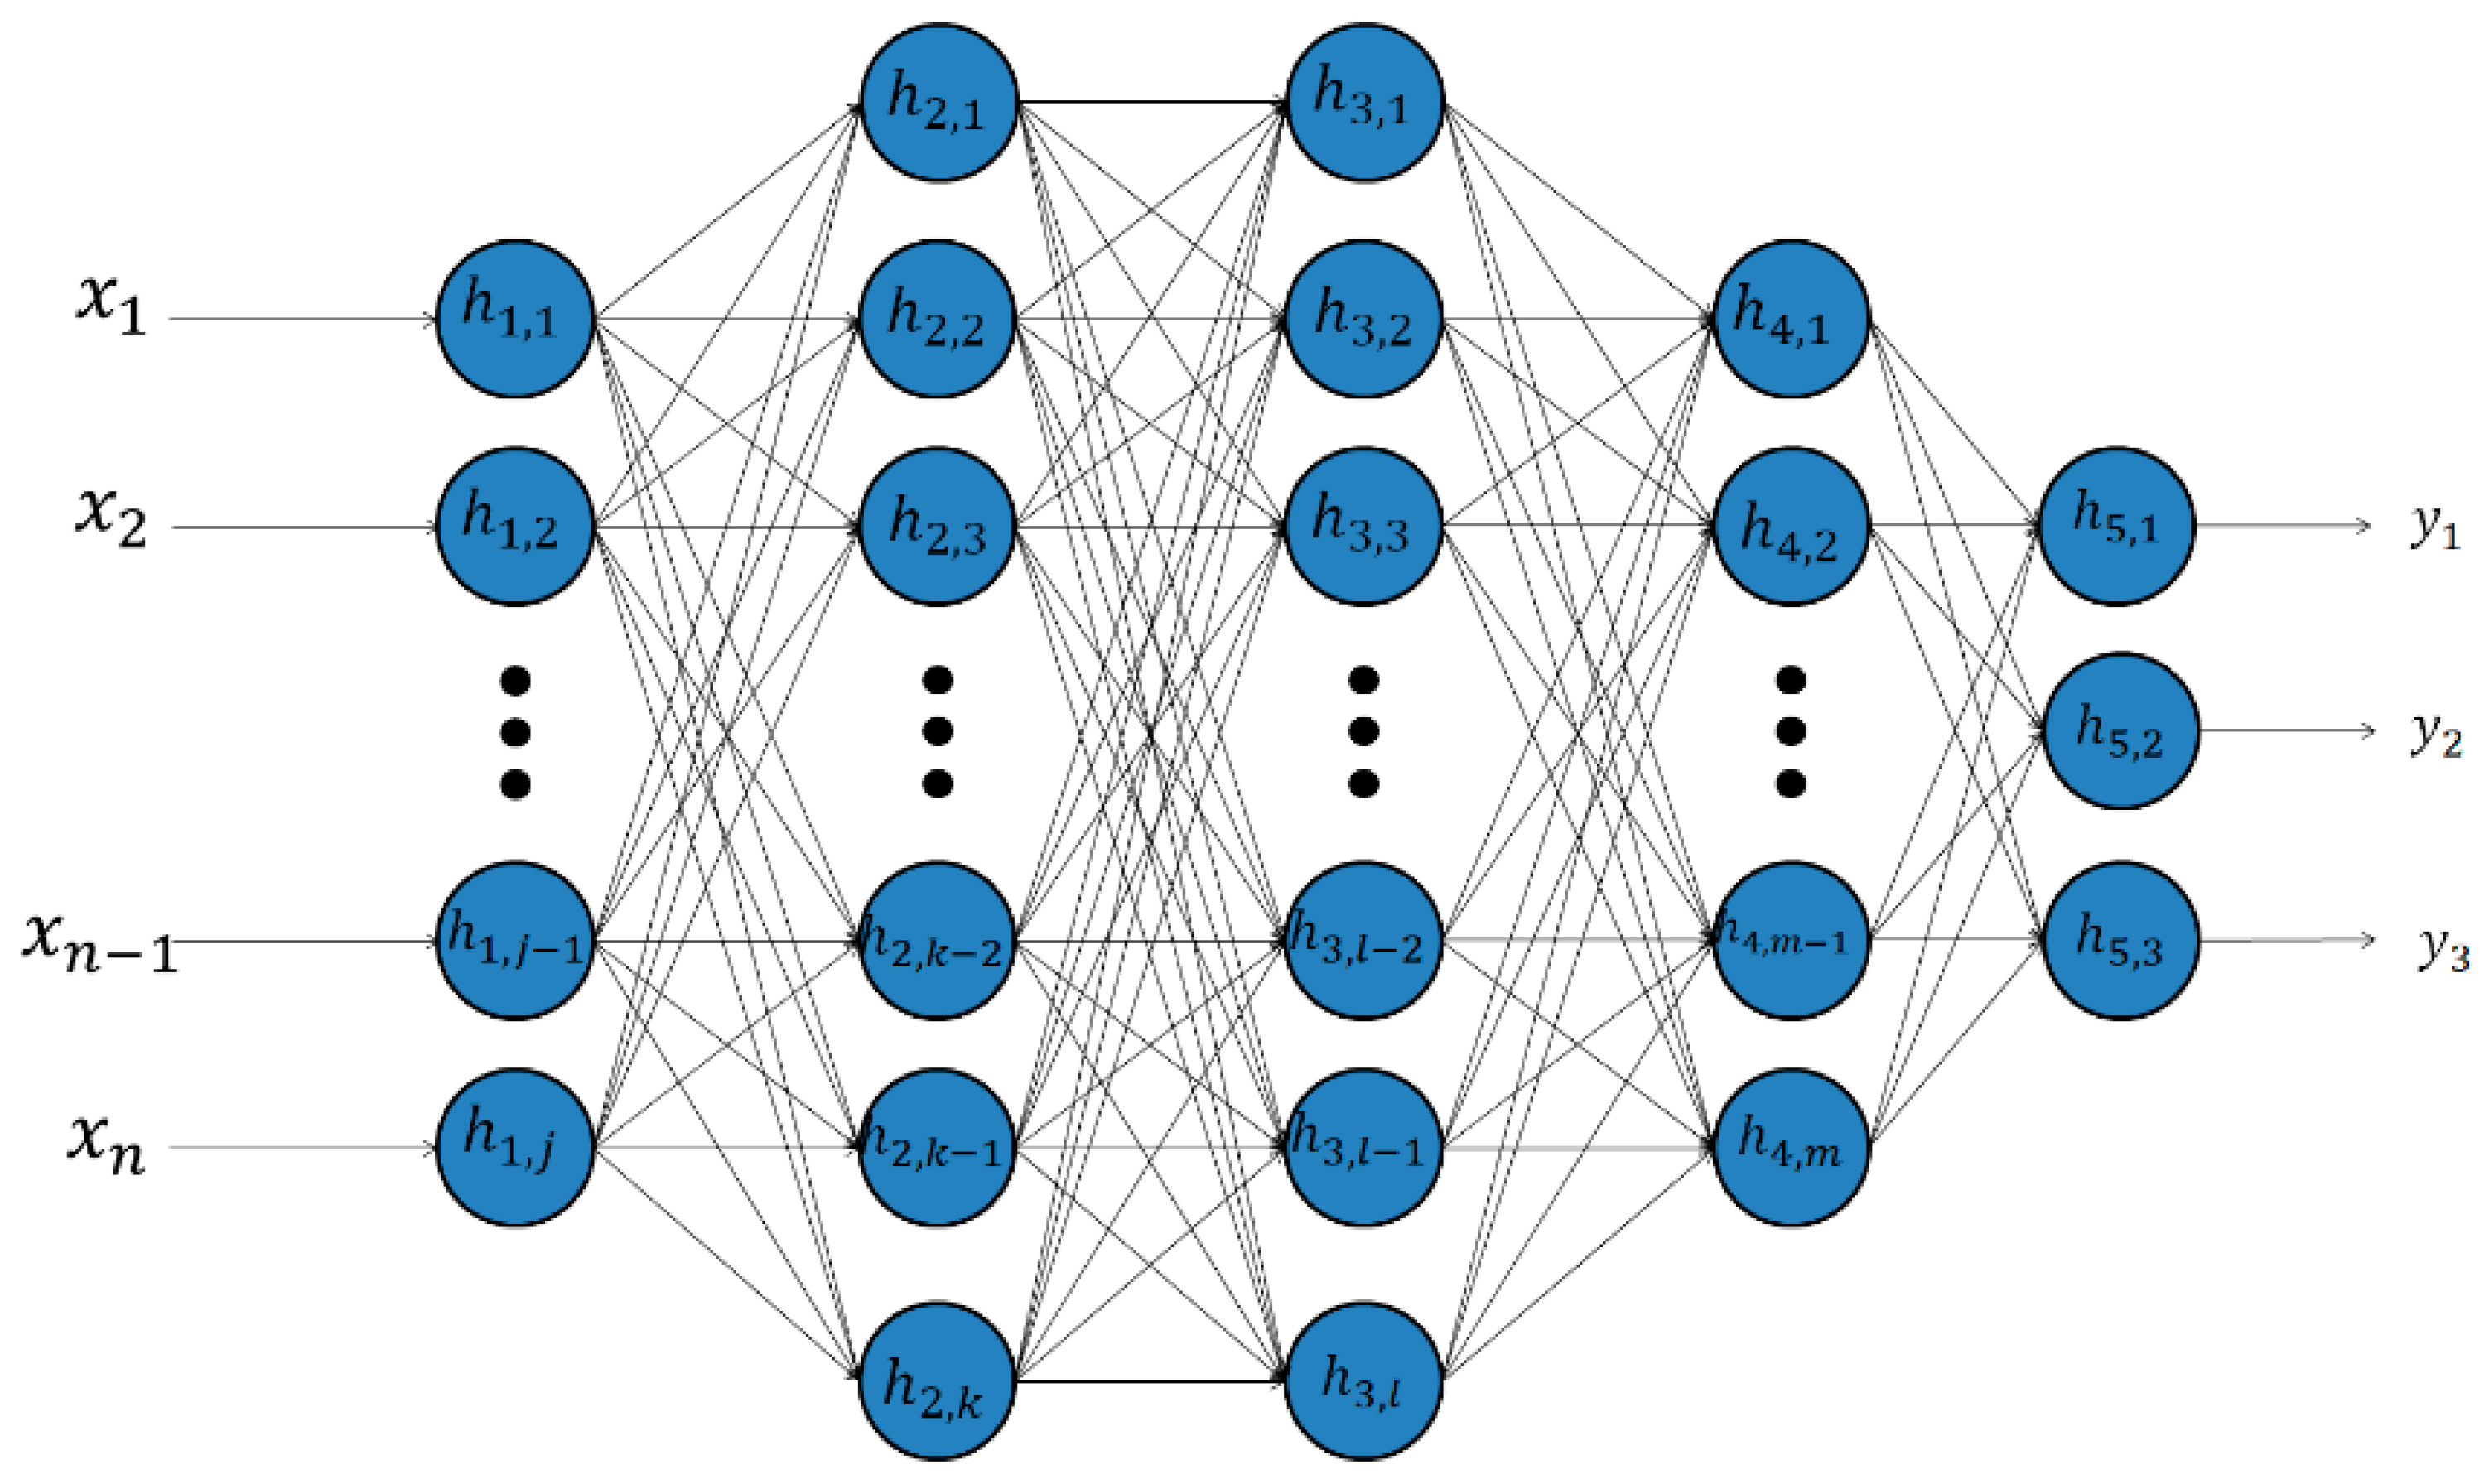
\includegraphics[width=\linewidth]{figures/ann.jpg}}
        \caption{Visual representation of an artificial neural network \cite{article:18}.}
        \label{fig:ann}
    \end{figure}

    \subsubsection{Convolutional neural network}
    A convolutional neural network (CNN) is a supervised artificial neural network that can process multidimensional inputs such as images or spectrograms of audio \cite{lecun1995convolutional}.
    This network combines convolutional and pooling layers for feature extraction with an ANN for final classification, see Fig. \ref{fig:cnn}.
    CNN works by shifting a filter across the input, computing a dot product and passing the output to an activation function.
    The pooling layers perform non-linear downsampling to reduce the size of feature maps and the number of trainable parameters.
    Pooling layers occur multiple times in the architecture following one or more convolutional layers.
    The training works in a similar manner to conventional ANNs by using the gradient descent algorithm and backpropagation.
    Convolutional neural networks have a broad range of applications, such as image and audio processing, object recognition and anomaly detection.

    \begin{figure}[htbp]
        \centerline{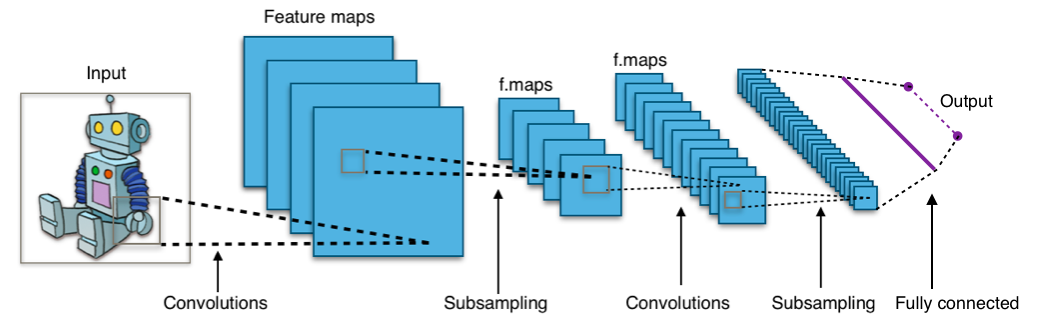
\includegraphics[width=\linewidth]{figures/cnn2.png}}
        \caption{Visual representation of a convolutional neural network \cite{ConvNet}.}
        \label{fig:cnn}
    \end{figure}

    \subsubsection{Deep autoencoder}
    Autoencoder is an unsupervised artificial neural network that learns to compress and reconstruct the input \cite{ballard1987modular}, \cite{rumelhart1985learning}.
    It consists of an encoder and decoder part, as depicted in Fig. \ref{fig:ae}.
    The encoder is an ANN in which each hidden layer is smaller than the preceding one.
    The objective of the encoder is to learn a low-dimensional representation of the input data.
    The decoder is an ANN that performs up-sampling of input data back to its original size.
    The training takes place in the same manner as conventional ANN, but it does not require labelled training data.
    Autoencoders find use in anomaly detection, facial recognition and image processing.

    \begin{figure}[htbp]
        \centerline{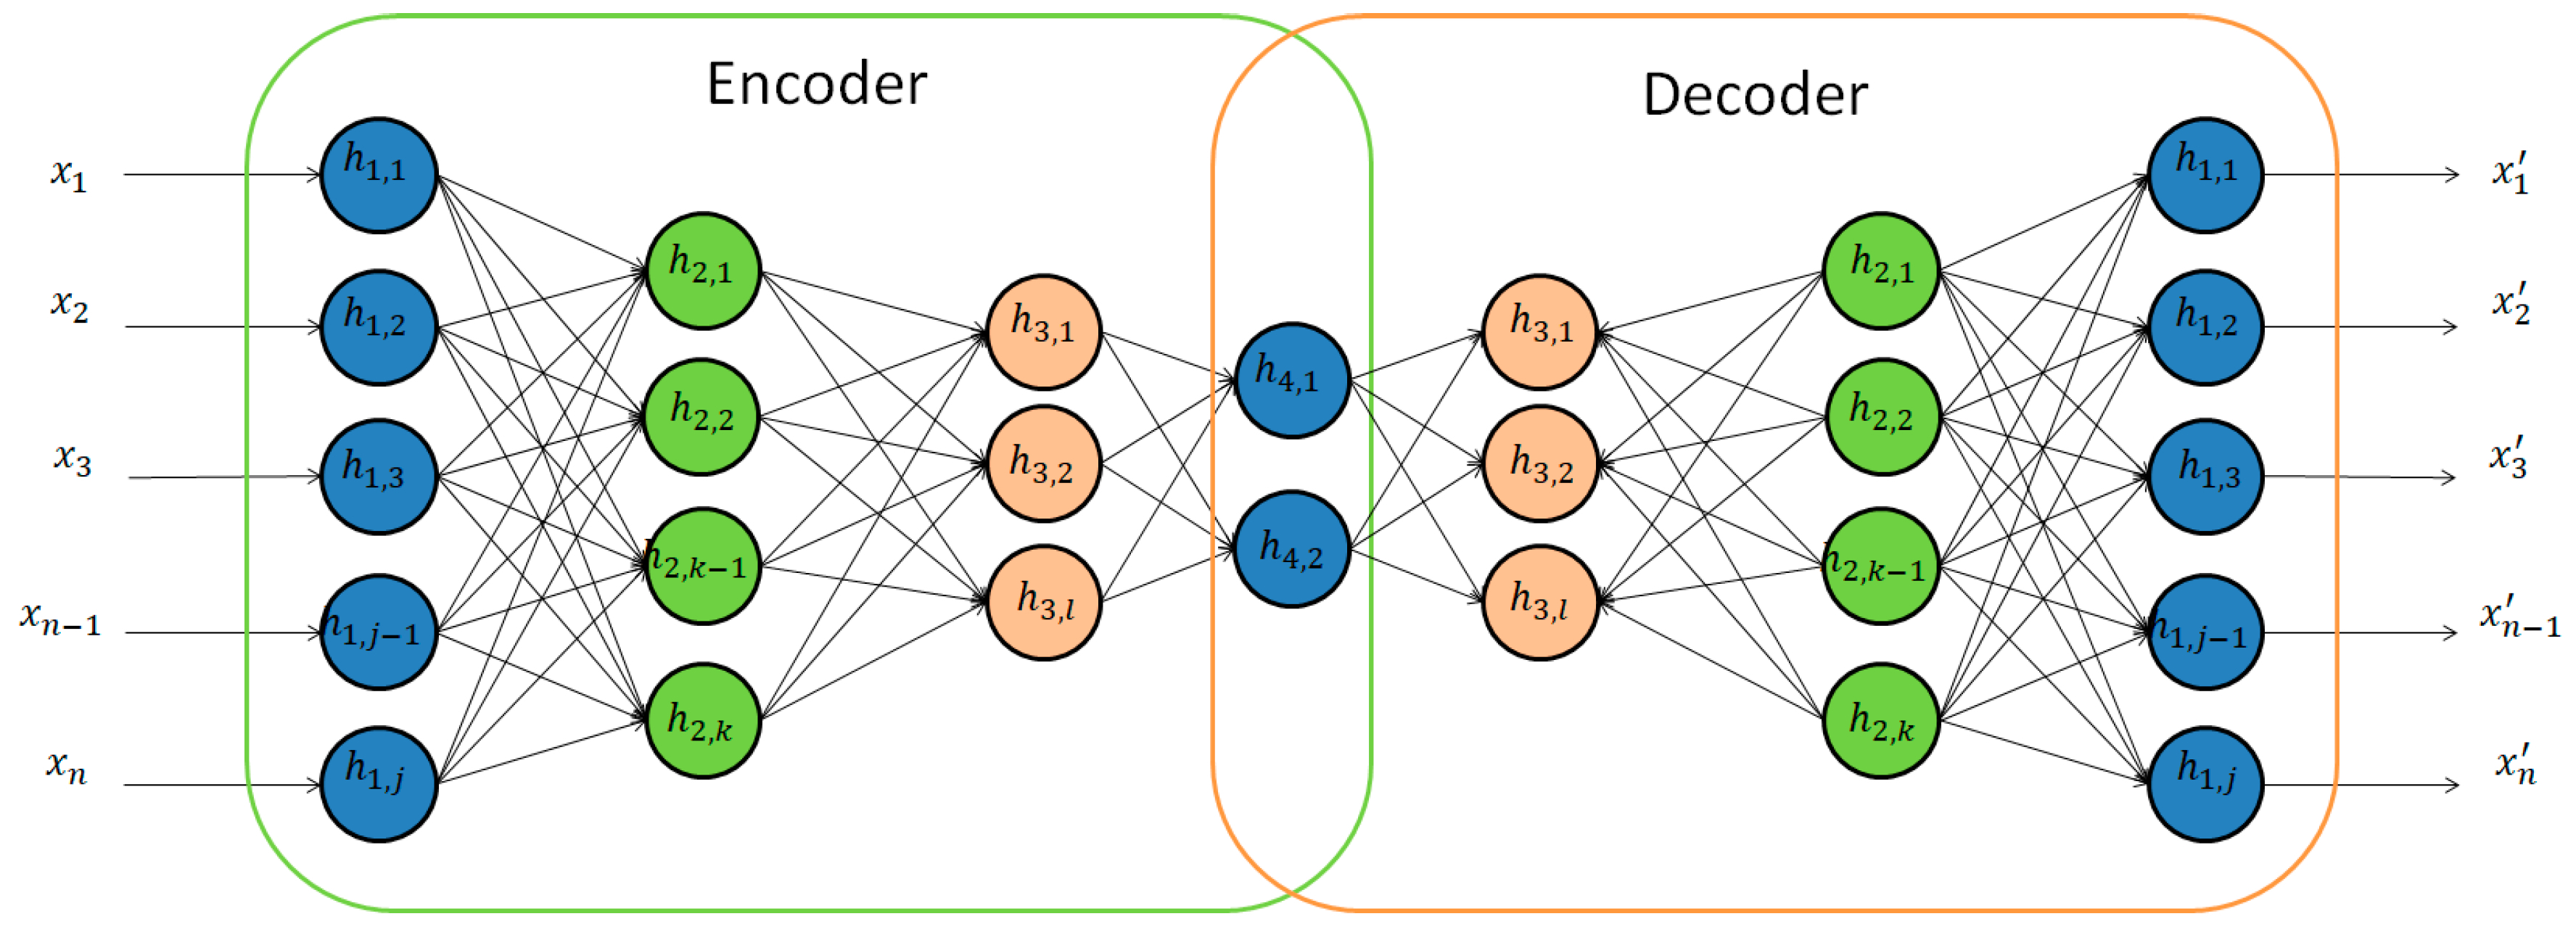
\includegraphics[width=\linewidth]{figures/ae.jpg}}
        \caption{Visual representation of an autoencoder \cite{article:18}.}
        \label{fig:ae}
    \end{figure}

    \subsubsection{Performance metrics}
    There are different metrics for describing the performance of machine learning and deep learning models depending on the nature of the classification task \cite{Goodfellow-et-al-2016}, \cite{sokolova2009systematic}, \cite{garcia2009study} .
    Accuracy, precision, recall, F1 score and area under the curve (AUC) evaluate the performance of binary classification \cite{sokolova2009systematic}.
    In the case of multi-class problems, the researchers use accuracy and Cohen's Kappa \cite{garcia2009study}.
    Derivation of these values is possible by the setting of a confusion matrix, see Table \ref{tab:cm}.
    The primary performance indicator among the reviewed studies is accuracy, which is the ratio of correctly classified examples among all examples.
    Comparison of machine learning models based solely on accuracy is only valid if all models in the publications use identical data for training and testing.
    \begin{table}[htbp]
        \begin{tabular}{l|l|c|c|c}
            \multicolumn{2}{c}{} & \multicolumn{2}{c}{True} & \\
            \cline{3-4}
            \multicolumn{2}{c|}{} & Positive & Negative & \multicolumn{1}{c}{Total} \\
            \cline{2-4}
            \multirow{2}{*}{Predicted} & Positvive                 & $a$                       & $b$                       & $a+b$                   \\
            \cline{2-4}
            & Negative                  & $c$                       & $d$                       & $c+d$                   \\
            \cline{2-4}
            \multicolumn{1}{c}{}       & \multicolumn{1}{c}{Total} & \multicolumn{1}{c}{$a+c$} & \multicolumn{    1}{c}{$b+d$} & \multicolumn{1}{c}{$N$}\\
        \end{tabular}
        \caption{Confusion matrix.}
        \label{tab:cm}
    \end{table}

    \subsection{Methods}
    Machine learning methods for DDoS detection can be classified into two classes based on where the inference takes place:

    \subsubsection{On-device detection}
    In \cite{article:7}, the authors propose a novel approach for malware detection on IoT devices.
    They convert a binary malware executable file into an 8-bit vector and visualize it as fixed width, variable height grayscale image.
    They observe that images of files from different malware families appear visually distinct from malware files belonging to the same family.
    Based on their findings, they extract features from the image using GIST, which has proven successful for scene and object classification tasks \cite{torralba2003context}.
    The authors use a steerable pyramid, a multi-scale and multi-orientation image representation technique that applies multiple subsampling and smoothing stages resulting in a structure similar to a pyramid.
    For the classification, they use an unsupervised k-nearest neighbours algorithm.
    The k-nearest neighbour's method leverages the existing data for clustering based on a similarity metric, for example, Euclidean distance \cite{taunk2019brief}.
    The classification of previously unseen samples takes place by feature extraction and selection of the k-nearest neighbours of that sample.
    The prediction is the majority of selected neighbours' labels.
    The authors evaluate the detection performance on a larger dataset of 25 different malware families comprising 9,458 binaries and tenfold cross-validation.
    Each evaluation uses a randomly sampled subset of data for the train (90\%) and test (10\%) sets.
    The results show that their method achieves similar classification performance to related work but is about 40 times faster.
    K-nearest neighbour algorithm requires storing the malware data in memory, rendering it ineffective for running on IoT devices.
    In \cite{article:3}, the authors use the visual representation of malware binaries and provide a resource-efficient classifier specifically for IoT devices.
    They convert malware binaries to grayscale images and leverage a small-size convolutional neural network for classification.
    The advantage of neural networks is that they automatically extract non-linear features from data.
    The resource-consuming training process takes place in the cloud environment, which is beneficial since the device does not have to store data compared to the k-nearest neighbours' algorithm.
    The resource-constrained devices receive a pre-trained model and perform the classification locally.
    In the study, the authors propose using a two-tier architecture combining a lightweight, on-device classifier with a powerful cloud-based one.
    In this case, the objective is to recognize suspicious programs locally on the device and hand them over to the backend server for further analysis.
    The researchers conduct experiments using the IoT DDoS malware dataset IoTPOT \cite{IoTPOT}.
    The dataset consists of 500 malware examples from multiple malware families.
    They collect the same number of samples of benign software to augment the data and divide the resulting data into train and test sets.
    They train their model to differentiate between goodware and malware and perform five-fold cross-validation.
    They show that the model detects malware with about 94\% accuracy while having the least amount of parameters compared to models from other studies.
    As future improvements, they suggest further optimization of the network in terms of performance by reducing the network size.

    \begin{figure}[htbp]
        \centerline{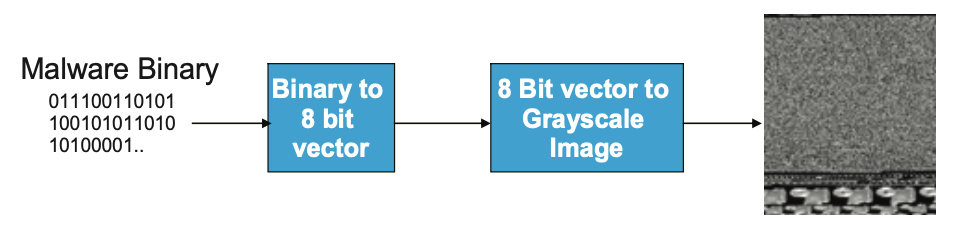
\includegraphics[width=\linewidth]{figures/malware-to-gray.png}}
        \caption{Converting malware binary to a grayscale image.}
        \label{fig1}
    \end{figure}

    \begin{figure*}[htbp]
        \begin{subfigure}{0.31\textwidth}
            \centerline{
\includegraphics[width=\linewidth]{figures/mirai-malware.png}}
            \caption{Mirai family}
            \label{fig2a}
        \end{subfigure}%
        \hspace*{\fill}
        \begin{subfigure}{0.31\textwidth}
            \centerline{
\includegraphics[width=\linewidth]{figures/gafgyt-malware.png}}
            \caption{Gafgyt family}
            \label{fig2b}
        \end{subfigure}%
        \hspace*{\fill}
        \begin{subfigure}{0.31\textwidth}
            \centerline{
\includegraphics[width=\linewidth]{figures/goodware.png}}
            \caption{Goodware}
            \label{fig2c}
        \end{subfigure}%
        \caption{Example of malware and goodware binaries represented as grayscale images \cite{article:7}.}
        \label{fig2}
    \end{figure*}

    \subsubsection{Network-based detection}
    In \cite{article:4}, the authors propose a network-based approach that uses a deep learning model for anomaly detection in an enterprise network scenario.
    The detection leverages statistical features of benign IoT traffic such as packet Source IP address, MAC address, packet size, etc.
    It works by monitoring each device's traffic in the network and inspecting packets within different time window periods, for example, 100ms, 500ms, etc.
    Each host has a dedicated model to detect anomalous and suspicious behaviour.
    The benefit of this approach is a high heterogeneity tolerance considering the diversity of IoT hardware and functionality.
    Additionally, the detection runs on a dedicated host, so IoT devices do not require additional computation, memory and energy.
    Since model training and inference take place in the enterprise environment, the detection algorithm uses actual traffic data to learn.
    The proposed approach consists of four phases: data collection, feature extraction, training, and monitoring.
    First, the authors obtain the raw network data by monitoring organizational traffic using Wireshark.
    They ensure the collected data is clean by starting the capturing process immediately after the device installation and include traffic data of frequent (data transmission) and infrequent (booting) actions.
    They create a snapshot of 115 statistics describing the traffic from or to the device.
%    They use a deep autoencoder architecture for anomaly detection.
%    An autoencoder is an unsupervised deep learning model for learning efficient encodings of unlabelled input data.
%    The model works by compressing the data into a reduced-size latent space and reconstructing the input.
%    The training objective is to minimize the error between the input and output.
%    Autoencoders usually perform applications such as dimensionality reduction, image compression, image denoising, anomaly detection and machine translation.
    The study uses an autoencoder to reconstruct benign instances of network behaviour traffic.
    When a device exhibits abnormal behaviour, the reconstruction will fail accordingly.
    They create a separate model for each device in the network and perform hyperparameter optimization, respectively.
    They use the mean square error between the model's input and the reconstructed output as their cost function.
    After the training, they determine a threshold for when the reconstructed instance is considered anomalous.
    Preliminary experiments show a high detection rate but often cause false alarms.
    The solution is to compute the detection based on the majority of votes over a sliding window to decide if the whole stram is benign or anomalous.
    For the model evaluation, the authors infect nine different manufacturer devices with BASHLITE and MIRAI botnets and monitor the network.
    Furthermore, the authors use the same traffic data to train three other commonly used anomaly detection algorithms and compare the results.
    The comparison reveals that autoencoder has the lowest ratio of false positives and requires the least time to perform detection.
    The weakness of this study is the difficulty of capturing diversified data for devices with broad functionalities.
    Future improvements include transfer learning that would allow re-using models pre-trained in other organizations to save time or support devices before connecting them to the enterprise network.


    \section{Discussion}
    Machine learning and deep learning offer significant improvements over conventional DDoS detection methods and facilitate applications such as anomaly and on-device malware detection \cite{article:15}.
    It is hard to compare the accuracy of individual studies because they use different datasets and various lab setups to generate data.
    The literature reviewed in this study shows machine learning and deep learning models have great potential for DDoS detection in IoT.
    The majority of studies focus on network-level anomaly detection by leveraging metadata of traffic flow.
    Table \ref{tab1} contains a summary and comparative analysis of the reviewed studies.
    Network-based anomaly detection is particularly beneficial for networks with resource-constrained devices that cannot execute complex software.
    Integration of network-based DDoS detection into existing networks offers an opportunity for an extra layer of security without the need to change the current infrastructure.
    One study shows that a deep learning-powered, network-based DDoS detection system is a viable, uncomplicated and provides a low-cost solution even within a home network \cite{inproceedings:1}.
    However, supervised learning approaches show limited potential for discovering unknown attacks.
    Furthermore, there is a limited amount of publicly available datasets to train supervised models.
    For this reason, the researchers set up their own IoT networks in a controlled environment and emulate a DDoS attack using a known malware such as Mirai.

    The low availability of actual DDoS data for supervised algorithms puts unsupervised learning techniques in favour \cite{xin2018machine}.
    Unsupervised learning approaches demonstrate an opportunity for using machine learning algorithms without labelled data.
    Integration of this approach is more complicated than using an existing dataset because the data has to exhibit all legitimate traffic patterns for each device in the network.
    However, transfer learning could provide a viable solution by supplying pre-trained models for each device.
    This way, existing networks could integrate DDoS detection without knowledge about machine learning and changes in the infrastructure.
    Transfer learning provides an opportunity for further research on on-device inference, which has to consider hardware limitations and energy consumption of IoT devices.
    Researchers in \cite{article:3} proved the capabilities of running a lightweight deep learning algorithm for malware detection on an IoT device.
    An opportunity for further research is to examine autoencoder-based anomaly detection techniques on-device.
    Studies report the solid performance of conventional machine learning techniques in the field of cyber-security \cite{xin2018machine}.
    The drawback of these approaches is their limited ability to generalise information to classify previously unseen examples and the requirement for manual feature engineering \cite{Goodfellow-et-al-2016}.
    Deep learning models outperform conventional machine learning in computer vision and natural language processing \cite{Goodfellow-et-al-2016}.
    However, their effectiveness strongly depends on the availability of high-quality cyber-security datasets.
    Deep learning critics emphasise privacy issues, the difficulty diagnosing errors and computational complexity.
    Regulatory approaches for forcing device manufacturers to implement security measures and updates for their devices are necessary.
    However, the legal process takes a long time and is not considered a short-term solution.
    Providing the highest level of DDoS protection for IoT requires a combination of regulatory, prevention and detection approaches.

    \begin{table*}[htbp]
        \caption{Comparison of machine learning algorithms for DDoS detection}
        \begin{center}
            \makegapedcells
            \begin{tabularx}{\linewidth}{|l|X|X|X|}
                \hline
                \multicolumn{1}{|c|}{\textbf{Methods}}                              & \multicolumn{1}{|c|}{\textbf{Working principle}}                                                                                                                                                     & \multicolumn{1}{|c|}{\textbf{Advantages}}                                                                                   & \multicolumn{1}{|c|}{\textbf{Disadvantages}} \\
                \hline
                Convolutional Neural Network \cite{article:3}                       & Convert malware binaries to grayscale image, apply CNN classifier, send suspicious binaries for deeper analysis to a backend server & Lightweight architecture, runs on device with high accuracy, trained with actual malware data, detects variants of malware from same family                   & Encryption and obfuscation might avoid detection, two tier-architecture, benign binaries vary between operating systems and CPU architectures                \\
                \hline
                K-nearest neighbours \cite{article:7}                               & Convert malware binaries to grayscale image, use feature extraction, detection based on clustering on device or a backend server & Simple and fast, high accuracy, trained with actual malware data, detects variants of malware from same family                  & Requires storing of the data on IoT device so might be not feasible for IoT devices, encryption and obfuscation might avoid detection, benign binaries vary between operating systems and CPU architectures                      \\
                \hline
                Artificial Neural Network \cite{article:13}, \cite{inproceedings:1} & Uses packet header metadata as input, once trained the traffic is monitored and when thresholds for packet number is exceeded the model classifies traffic as anomalous or not & Detects known and unknown attacks with high accuracy                   & Cannot detect when packet headers are encrypted                      \\
                \hline
                Boosting (LMT) \cite{article:10}                                    & Has two classifiers. One assigns device to pre-defined classes. The other detects DDoS attack based on traffic data and device profile class & By using device profile groups there's no requirement for individual DDoS detection models per device                   & Requires models for device profile assignment and DDoS detection, device profiling uses complex feature selection, high storage requirement                      \\
                \hline
                Autoencoder \cite{article:4}                                        & Works by reconstructing packets originating from IoT device. If the autoencoder is unable to reconstruct the input it indicates abnormal device activities & Has a low false-positive rate compared to other approaches, does not require a dataset it works by learning patterns in live data, the detection time is lower than alternative approaches. It can detect novel and zero-day attacks    & Requires a model per device, the performance was evaluated with simulated data, complicated to train properly if a device has wide range of functions and infrequent traffic patterns                      \\
                \hline
            \end{tabularx}
            \label{tab1}
        \end{center}
    \end{table*}


    \section{Conclusion}
    This study provides a comprehensive overview of machine learning methods for DDoS detection in the IoT and summarizes their primary methods, functioning, benefits and critics.
    It starts by introducing IoT architecture, DDoS, botnets and machine learning, followed by a detailed explanation of two deep learning approaches.
    DDoS detection in IoT combines diverse subjects, including botnet, malware and anomaly detection.
    Current works show great potential for deep learning algorithms, although there remains room for improvement, particularly in on-device inference and availability of actual DDoS data.
    Further research will benefit from experts in multiple research fields, including cyber-security, machine learning and networking.


%    \newpage
%    \nocite{*}
    \bibliographystyle{ieeetr}
    \bibliography{refs}

\end{document}
